\documentclass[tikz,border=6pt]{standalone}
\usepackage[T1]{fontenc}
\usepackage[utf8]{inputenc}
\usepackage{pgfplots}
\usepgfplotslibrary{groupplots}
\usetikzlibrary{calc}
\pgfplotsset{compat=1.18}
\begin{document}
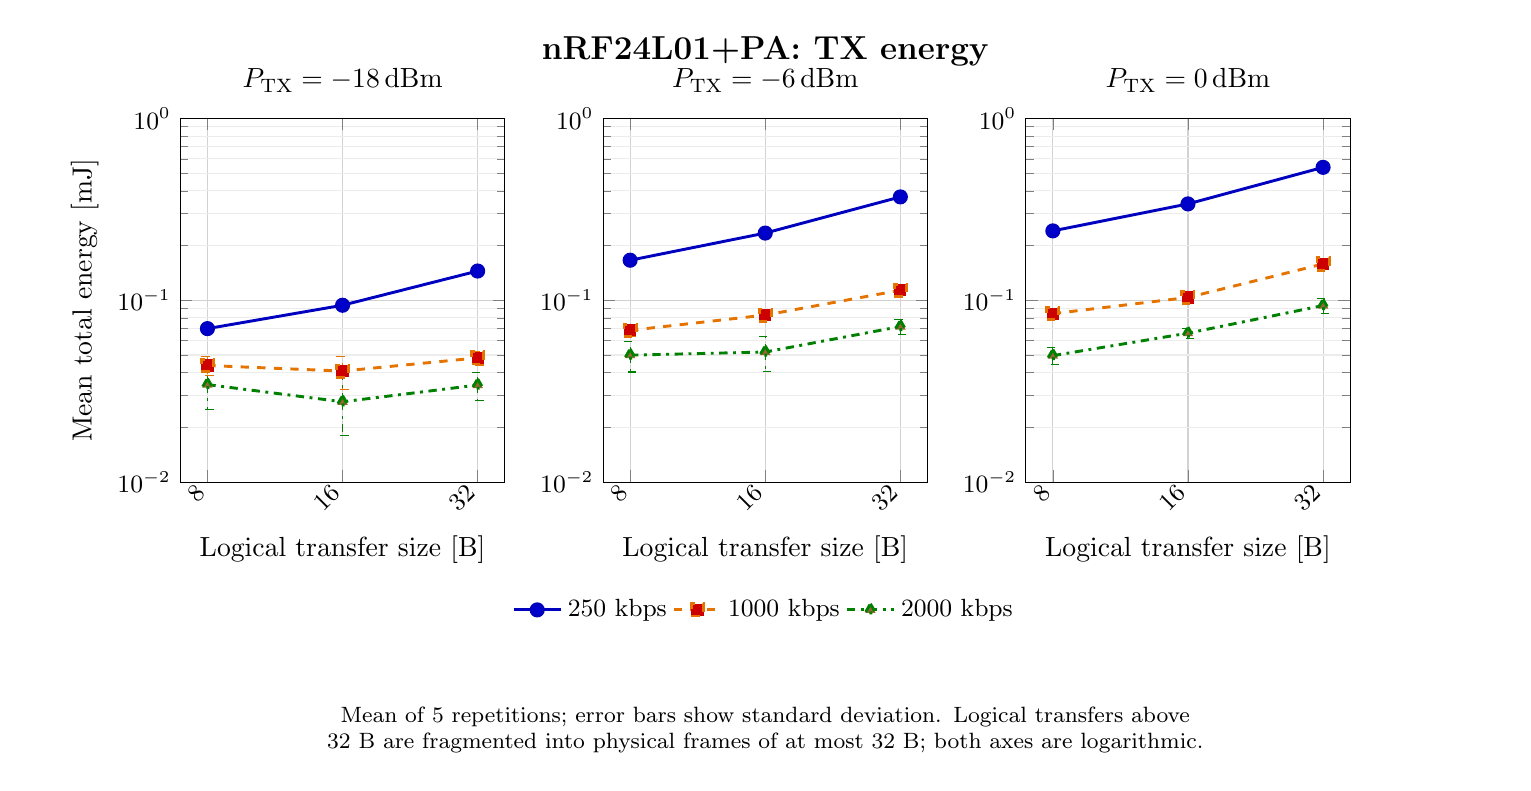
\begin{tikzpicture}
\begin{groupplot}[/pgf/number format/use comma,
  group style={group size=3 by 1, horizontal sep=1.25cm},
  width=5.7cm, height=6.2cm,
  xmode=log, log basis x={2}, ymode=log, log basis y={10},
  ymin=0.01, ymax=1,
  xtick={8,16,32}, xticklabels={8,16,32},
  x tick label style={rotate=45, anchor=east, font=\small},
  y tick label style={font=\small},
  grid=both, minor grid style={gray!15}, major grid style={gray!35},
  xlabel={Logical transfer size [B]},
  every axis plot/.append style={line width=1.05pt},
  error bars/error bar style={line width=0.35pt},
  legend style={font=\small, draw=none, fill=none, at={(0.5,-0.29)},
    anchor=north, legend columns=-1},
]
\nextgroupplot[title={\(P_{\mathrm{TX}}=-18\,\mathrm{dBm}\)}, ylabel={Mean total energy [mJ]}]
\addplot+[
  color=blue!75!black, solid, mark=*, mark size=2.2pt,
  error bars/.cd, y dir=both, y explicit,
] coordinates {
  (8,0.0698373524) +- (0,0.00143509994)
  (16,0.093887224) +- (0,0.000494825132)
  (32,0.144839559) +- (0,0.000548143344)
};
\addplot+[
  color=orange!90!black, dashed, mark=square*, mark size=2.2pt,
  error bars/.cd, y dir=both, y explicit,
] coordinates {
  (8,0.0437897431) +- (0,0.00518993626)
  (16,0.0408023352) +- (0,0.00842724654)
  (32,0.0482069695) +- (0,0.0041603537)
};
\addplot+[
  color=green!50!black, dashdotted, mark=triangle*, mark size=2.2pt,
  error bars/.cd, y dir=both, y explicit,
] coordinates {
  (8,0.0343793658) +- (0,0.00920099947)
  (16,0.0276515788) +- (0,0.00969298034)
  (32,0.0341946997) +- (0,0.00609808335)
};
\nextgroupplot[title={\(P_{\mathrm{TX}}=-6\,\mathrm{dBm}\)}]
\addplot+[
  color=blue!75!black, solid, mark=*, mark size=2.2pt,
  error bars/.cd, y dir=both, y explicit,
] coordinates {
  (8,0.166064835) +- (0,0.00266901629)
  (16,0.23418549) +- (0,0.00161803334)
  (32,0.370331294) +- (0,0.00123075885)
};
\addlegendentry{250 kbps}
\addplot+[
  color=orange!90!black, dashed, mark=square*, mark size=2.2pt,
  error bars/.cd, y dir=both, y explicit,
] coordinates {
  (8,0.0683167046) +- (0,0.00501017963)
  (16,0.082929494) +- (0,0.00542103887)
  (32,0.113584017) +- (0,0.00607304743)
};
\addlegendentry{1000 kbps}
\addplot+[
  color=green!50!black, dashdotted, mark=triangle*, mark size=2.2pt,
  error bars/.cd, y dir=both, y explicit,
] coordinates {
  (8,0.0499085791) +- (0,0.00961159738)
  (16,0.0519381323) +- (0,0.0115585368)
  (32,0.0717292638) +- (0,0.00696853952)
};
\addlegendentry{2000 kbps}
\nextgroupplot[title={\(P_{\mathrm{TX}}=0\,\mathrm{dBm}\)}]
\addplot+[
  color=blue!75!black, solid, mark=*, mark size=2.2pt,
  error bars/.cd, y dir=both, y explicit,
] coordinates {
  (8,0.240757209) +- (0,0.00285552535)
  (16,0.338846214) +- (0,0.0019304071)
  (32,0.538376496) +- (0,0.00213679928)
};
\addplot+[
  color=orange!90!black, dashed, mark=square*, mark size=2.2pt,
  error bars/.cd, y dir=both, y explicit,
] coordinates {
  (8,0.0843866627) +- (0,0.00496314984)
  (16,0.103627102) +- (0,0.00632496032)
  (32,0.158349521) +- (0,0.00454069624)
};
\addplot+[
  color=green!50!black, dashdotted, mark=triangle*, mark size=2.2pt,
  error bars/.cd, y dir=both, y explicit,
] coordinates {
  (8,0.0495938279) +- (0,0.00535509862)
  (16,0.0659304848) +- (0,0.00400478031)
  (32,0.0935441755) +- (0,0.00852946989)
};
\end{groupplot}
\node[font=\bfseries\large] at ($(group c2r1.north)+(0,0.85cm)$)
  {nRF24L01+PA: TX energy};
\node[font=\footnotesize, align=center, text width=18.5cm]
  at ($(group c2r1.south)+(0,-3.15cm)$)
  {Mean of 5 repetitions; error bars show standard deviation. Logical transfers above 32 B are fragmented into physical frames of at most 32 B; both axes are logarithmic.};
\end{tikzpicture}
\end{document}
